\documentclass[runningheads,a4paper]{llncs}

\usepackage[american]{babel}

\usepackage{graphicx}

%extended enumerate, such as \begin{compactenum}
\usepackage{paralist}

%put figures inside a text
%\usepackage{picins}
%use
%\piccaptioninside
%\piccaption{...}
%\parpic[r]{\includegraphics ...}
%Text...

%Sorts the citations in the brackets
%\usepackage{cite}

%for easy quotations: \enquote{text}
\usepackage{csquotes}

\usepackage[T1]{fontenc}

%enable margin kerning
\usepackage{microtype}

%better font, similar to the default springer font
\usepackage[%
rm={oldstyle=false,proportional=true},%
sf={oldstyle=false,proportional=true},%
tt={oldstyle=false,proportional=true,variable=true},%
qt=false%
]{cfr-lm}
%
%if more space is needed, exchange cfr-lm by mathptmx
%\usepackage{mathptmx}

%for demonstration purposes only
\usepackage[math]{blindtext}

\usepackage[
%pdfauthor={},
%pdfsubject={},
%pdftitle={},
%pdfkeywords={},
bookmarks=false,
breaklinks=true,
colorlinks=true,
linkcolor=black,
citecolor=black,
urlcolor=black,
%pdfstartpage=19,
pdfpagelayout=SinglePage
]{hyperref}
%enables correct jumping to figures when referencing
\usepackage[all]{hypcap}

\usepackage{url}

\usepackage[table,xcdraw]{xcolor}
\usepackage{footnote}



\usepackage[capitalise,nameinlink]{cleveref}
%Nice formats for \cref
\crefname{section}{Sect.}{Sect.}
\Crefname{section}{Section}{Sections}
\crefname{figure}{Fig.}{Fig.}
\Crefname{figure}{Figure}{Figures}

\usepackage{xspace}
%\newcommand{\eg}{e.\,g.\xspace}
%\newcommand{\ie}{i.\,e.\xspace}
\newcommand{\eg}{e.\,g.,\ }
\newcommand{\ie}{i.\,e.,\ }

%introduce \powerset - hint by http://matheplanet.com/matheplanet/nuke/html/viewtopic.php?topic=136492&post_id=997377
\DeclareFontFamily{U}{MnSymbolC}{}
\DeclareSymbolFont{MnSyC}{U}{MnSymbolC}{m}{n}
\DeclareFontShape{U}{MnSymbolC}{m}{n}{
    <-6>  MnSymbolC5
   <6-7>  MnSymbolC6
   <7-8>  MnSymbolC7
   <8-9>  MnSymbolC8
   <9-10> MnSymbolC9
  <10-12> MnSymbolC10
  <12->   MnSymbolC12%
}{}
\DeclareMathSymbol{\powerset}{\mathord}{MnSyC}{180}

%improve wrapping of URLs - hint by http://tex.stackexchange.com/a/10419/9075
\makeatletter
\g@addto@macro{\UrlBreaks}{\UrlOrds}
\makeatother

% correct bad hyphenation here
\hyphenation{op-tical net-works semi-conduc-tor}

\begin{document}

%Works on MiKTeX only
%hint by http://goemonx.blogspot.de/2012/01/pdflatex-ligaturen-und-copynpaste.html
%also http://tex.stackexchange.com/questions/4397/make-ligatures-in-linux-libertine-copyable-and-searchable
%This allows a copy'n'paste of the text from the paper
\input glyphtounicode.tex
\pdfgentounicode=1

\title{Technology Support in Smart City Learning:\\ a Mapping of the Literature}
%If Title is too long, use \titlerunning
%\titlerunning{Short Title}

%Single insitute
\author{Francesco Gianni \and Monica Divitini\\
francesco.gianni@idi.ntnu.no, monica.divitini@idi.ntnu.no}
%If there are too many authors, use \authorrunning
%\authorrunning{First Author et al.}
\institute{Norwegian Univesity of Science and Technology\\
Department of Computer and Information Science\\
Trondheim, Norway}

%Multiple insitutes
%Currently disabled
%
\iffalse
%Multiple institutes are typeset as follows:
\author{Firstname Lastname\inst{1} \and Firstname Lastname\inst{2} }
%If there are too many authors, use \authorrunning
%\authorrunning{First Author et al.}

\institute{
Insitute 1\\
\email{...}\and
Insitute 2\\
\email{...}
}
\fi
			
\maketitle

\begin{abstract}
  With this literature mapping we want to know what type of research has been conducted in the area of technology-enhanced smart city learning. With smart city learning we refer to ...
\end{abstract}

%%\keywords{...}

%%%%%%%%%%%%%%%%%%%%%%%%%%%%%%%%%%%%%%%%%%%%%%%%%%%%%%%%%%%%%%%%%%%%%%%%%%%%%%%
\section{Introduction}\label{sec:intro}
The concept of smart-city has been used in many different context and is associated with distinctive and innovative aspects that are often quite different. Big diversities are observed on the reasons \textit{why} different cities are defined as \textit{smart}.

This situation is the consequence of the lack of a clear and recognized definition of smart city.

In attempting to pin down what is smart about the smart city, one finds that not only does it involve quite a diverse range of things (information technology, business innovation, governance, communities and sustainability) it can also be suggested that the label itself often makes certain assumptions about the relationship between these things for example regarding consensus and balance\cite{hollands_will_2008}.

Komninos\cite{komninos_intelligent_2002}, in his attempt to delineate the intelligent city, (perhaps the concept most closely related to the smart city), cites four possible meanings:

\begin{enumerate}
\item The application of a wide range of electronic and digital applications to communities and cities, which effectively work to conflate the term with ideas about the cyber, digital, wired, informational or knowledge\textendash based city.
\item The use of information technology to transform life and work within a region in significant and fundamental ways.
\item The meaning of intelligent or smart as embedded information and communication technologies in the city.
\item The spatial territories that bring ICTs and people together to enhance innovation, learning, knowledge and problem solving.
\end{enumerate}

Overall then, Komninos\cite{komninos_intelligent_2002} sees intelligent (smart) cities as ``\textit{territories with high capacity for learning and innovation, which is built\textendash in the creativity of their population, their institutions of knowledge creation, and their digital infrastructure for communication and knowledge management}''.

The adjective ``smart'' began to gain a increasingly notoriety between 2005 and 2007, when it started to be used to denote a sort of dream-city, i.e. a complex and optimized environment, or eco-system, where it could be desirable to live. It appeared immediately clear that the adjective smart was intended to go well beyond the meaning intelligent and/or to emphasize the use of IC and digital technologies\cite{giovannella_smart_2014-1}.

For this reason the authors chose to limit the search to articles published from 2005.

Smart cities are also a powerful ecosystem for learning. Smart city learning aim to support the improvement of all key factors contributing to the regional competitiveness: mobility, environment, people, quality of life and governance. The approach is aimed at optimizing resource consumption and saving time improving flows of people, goods and data\footnote{http://www.mifav.uniroma2.it/inevent/events/sclo/}.

Education in this context is pursued as a bottom-up process, where person and places are central. Smartness from a learning perspective exists both in the ambient data collected and among the communities that exists within a city.

The separation between student and teacher will fade out. Their role will be content or situation dependent: everybody will be a learner and the relation between persons will get a bigger role.

From the learning perspective, smart cities can be seen as an independent \textit{learning actor} that behaves like an autonomous entity which adapt itself in an evolving environment.

Despite this, the most interesting point of view for this work is probably the one that sees the smart city as a place where citizens learn smart-behaviours.

This scenario can involve traditional education which happens in facilities like schools and universities. The goal of this work is instead more oriented towards \textit{lifelong learning}, defined as the continuous build of skills to adapt and collaborate in dynamic ecosystems like smart cities.

\section{Motivation and Research Questions}
Technology in smart cities is essential and considered as a supporting backbone\cite{giovannella_smart_2014}.
The role of technology in smart cities has been widely recognized and addressed, however there seems to be no established field of research that connects smart cities to learning.

This work is motivated by the quest for a clear overview of existing research related to learning in smart cities.


\subsection{What do we consider as ``smart city learning''?} \label{subsec:definition}
Some of the studies that are situated in smart cities and also present a learning component take place in confined communities and facilities, like the elderly living in retirement houses or patients in hospitals. Even if these scenarios are physically situated in a (smart) city, they remain relevant and valid even if the smart city component is removed from the research context.

The \textit{smart city} term seems to be often attached to research works where it is not a central or absolutely essential element.

To avoid articles not relevant for the purpose of this work, the authors decided that the boundaries that define the adopted research scope on smart cities are dependent by two factors:

\begin{itemize}
\item The social perspective, which defines the people affected and should not be constrained by any particular bound. Every citizen can be involved.
\item The urban perspective, which includes the city as an urban space and it is not confined to any particular facility or environment that can be also found outside the smart city context.
\end{itemize}

A significant scenario should include at least one of the two factors. Here are some examples of scenarios:

\begin{enumerate}
\item Students collecting sensor data on their commute path to school or moving around the city. Data is then aggregated and presented to the community to facilitate reflection, learning and to stimulate sustainable and safer behaviors.
\item Citizens collecting energy consumption data in their house, which is then aggregated to create a energy consumption map for the whole city. Looking at the map, citizens can discover interesting patterns and reflect on the margin of improvement for their houses.
\item Bikes used for bike sharing services can be instrumented to collect air pollution and other sensor data. Cyclists around the city can provide a detailed and constantly updated sensor-map that can stimulate citizens to adopt more sustainable and efficient mobility patterns.
\end{enumerate}

All the three scenarios proposed are relevant for the smart city learning research scope defined above.

The first scenario works only within a defined community of citizens, but they are displaced in the entire urban environment of a smart city.

In the second scenario the space is confined into individual apartments and houses, but every citizen can be potentially involved. The data is also aggregated and interpreted at a city-wide level.

The third scenario combine both the social and urban perspective: there is no specific category of citizens being addressed and the relevant urban space is located in the city as a whole.


\subsection{Research Questions}
The research questions addressed are:

\begin{itemize}
\item \textbf{RQ1}: What are the main area of research within technology-enhanced smart city learning and where more research is needed? (technology enhanced learning approaches, personal, analytics, ecc)
\item \textbf{RQ2}: What technologies are used?
\item \textbf{RQ3}: Which learning theories and approaches are most commonly used in smart city learning? (situatedness, learning, collaboration, data collection, social interaction)
\item \textbf{RQ4}: What type of research is performed and which methods are used?
\item \textbf{RQ5}: How research on smart city learning has evolved in time?
\item \textbf{RQ6}: Which are the most common scenarios of application and usage setting?
\item \textbf{RQ7}: Is learning in smart city more oriented towards the city as a place where learning happens or as learning smart-behavior to improve lifestyle, participation and collaboration?
\item \textbf{RQ8}: Which kind of features and patterns characterize the technological applications used in SC?
\item \textbf{RQ9}: Where is research usually published?
\end{itemize}

\section{Data Sources and Search}
\subsection{Data Sources}
The articles were searched and collected using three different approaches:

\begin{enumerate}
\item keyword based search on different online databases
\item manual screening of selected conference proceedings
\item manual screening of selected special issues of journals
\end{enumerate}

The following online databases were used for the keyword based search:
\begin{itemize}
\item ISI Web of Science\footnote{https://apps.webofknowledge.com/}
\item ACM digital library\footnote{https://dl.acm.org/}
\item Elsevier - ScienceDirect\footnote{https://www.sciencedirect.com/}
\item Elsevier - Scopus\footnote{http://www.scopus.com/}
\item IEEE Xplore\footnote{http://ieeexplore.ieee.org/}
\end{itemize}

The following conference proceedings were searched for relevant articles:
\begin{itemize}
\item \textbf{CSCW} Computer-Supported Cooperative Work and Social Computing\footnote{http://cscw.acm.org/}
\item \textbf{CHI} Conference on Human Factors in Computing Systems\footnote{http://chiYYYY.acm.org/}
\item \textbf{EC-TEL} European Conference on Technology Enhanced Learning\footnote{http://www.ec-tel.eu/}
\item \textbf{AMI} International Joint Conference on Ambient Intelligence\footnote{http://www.ami-conferences.org/}
\item \textbf{C\&T} International Conference on Communities and Technologies\footnote{http://comtech.community/}
\end{itemize}

The following journal issues were searched for relevant articles:
\begin{itemize}
\item \textbf{IJDLDC} International Journal of Digital Literacy and Digital Competence vol. 3 n. 4 - Special Issue on \textit{``Smart City Learning, literacy and Competences''}\footnote{http://www.igi-global.com/journal/international-journal-digital-literacy-digital/1170}
\item \textbf{IxD\&A} Interaction Design and Architecture(s), vol. 16 (part I)\footnote{\url{http://www.mifav.uniroma2.it/inevent/events/idea2010/index.php?s=10&a=10&link=ToC_16_P}}, vol. 17 (part II)\footnote{\url{http://www.mifav.uniroma2.it/inevent/events/idea2010/index.php?s=10&a=10&link=ToC_17_P}} - Special Issue on \textit{``Smart City Learning - Visions and practical Implementations: toward Horizon 2020''} 
\end{itemize}

\subsection{Search and Keywords}
The keywords selection process was driven by the PICO framework. PICO helps to develop a comprehensive set of search keywords for quantitative research terms according to: Population, Intervention or Exposure (PECO), Comparison, Outcomes\cite{schardt_utilization_2007}.

Initially, keywords for all the sections of the framework were selected, but the authors decided later on to relax some constraints in order to avoid missing some possible relevant articles. A \textit{context} section was also added to the schema.

Table \ref{table:keywords} shows the PICO(C) structure with associated keywords.

%% table of keywords here
\begin{table}[ht]
\renewcommand{\arraystretch}{1.3}
\centering
\caption{PICO(C) Driven Keywords Framing}
\label{table:keywords}
\begin{tabular}{|
>{\columncolor[HTML]{EFEFEF}}l |l|}
\hline
\textbf{Population} & \textit{-} \\ \hline
\textbf{Intervention} & \textit{learning} \\ \hline
\textbf{Comparison} & \textit{-} \\ \hline
\textbf{Outcome} & \textit{\begin{tabular}[c]{@{}l@{}}participation, collaboration, reflection,\\ awareness\end{tabular}} \\ \hline
\textbf{Context} & \textit{\begin{tabular}[c]{@{}l@{}}cities, smart city, urban, connected city,\\ intelligent city, digital city\end{tabular}} \\ \hline
\end{tabular}
\end{table}

A pilot search was conducted on some of the online databases in order to refine the keywords and find a search query that could be adapted and used in all the different online databases.

The final search query used is reported in Table \ref{table:query}.

%% search query
\begin{table}[ht]
\renewcommand{\arraystretch}{1.3}
\centering
\caption{Search Query}
\label{table:query}
\begin{tabular}{c|c}
\rowcolor[HTML]{EFEFEF} 
\textbf{Context} & \begin{tabular}[c]{@{}c@{}}(cities OR "smart city" OR urban\\ OR "connected city" OR "intelligent city"\\ OR "digital city")\end{tabular} \\
 & \textbf{AND} \\
\rowcolor[HTML]{EFEFEF} 
\textbf{Intervention} & ("learning") \\
 & \textbf{AND} \\
\rowcolor[HTML]{EFEFEF} 
\textbf{Outcome} & \begin{tabular}[c]{@{}c@{}}(participation OR collaboration\\ OR reflection OR awareness)\end{tabular}
\end{tabular}
\end{table}

Different online databases offer different levels of search functionalities and details when going to use a complex query that possibly involves several keywords and fields (title, abstract, etc.).

Some of the difficulties encountered were:
\begin{itemize}
\item limit on the number of keywords that can be used;
\item limit on the fields where the search can be performed, search on title AND abstract not always possible;
\item no precise and direct control on the target search fields, keywords could be only searched on a preset aggregation of fields like title, abstract, article keywords;
\item different ways of coding the same logic expression, the same search string couldn't be reused on different databases;
\item different formats of the result set, in some cases was possible to batch-download the results, otherwise results had been scraped using Zotero\footnote{https://www.zotero.org/} browser integration.
\end{itemize}

The keywords were searched on title and abstract when possible, otherwise only the abstract was used. In Table \ref{table:result_1} the size of the result sets for each online database are outlined.

The articles collected were imported in a Zotero library, and duplicates were manually removed.

%% table of result count
\begin{savenotes}
\begin{table}[ht]
\setlength{\tabcolsep}{8pt}
\centering
\caption{Result Set for online databases before duplicates removal}
\label{table:result_1}
\begin{tabular}{cccccc|c}
 & \cellcolor[HTML]{EFEFEF}\textbf{ISI} & \cellcolor[HTML]{EFEFEF}\textbf{ACM} & \cellcolor[HTML]{EFEFEF}\textbf{ScienceDirect} & \cellcolor[HTML]{EFEFEF}\textbf{Scopus} & \cellcolor[HTML]{EFEFEF}\textbf{IEEE} & \textbf{TOT} \\
\textit{n} & 938 & 35 & 162 & 1022 & 42 & 2199 \\
\textit{field} & topic\footnote{Topic fields include Titles, Abstracts, Keywords and Indexing fields such as Systematics, Taxonomic Terms and Descriptors} & abstract & abstract & abstract & abstract & 
\end{tabular}
\end{table}
\end{savenotes}

%% table no duplicates
\begin{table}[ht]
\setlength{\tabcolsep}{8pt}
\centering
\caption{Final Result Set without duplicates and selected articles for coding}
\label{table:result_2}
\begin{tabular}{cccc|c}
 & \cellcolor[HTML]{EFEFEF}\textbf{Online Databases} & \cellcolor[HTML]{EFEFEF}\textbf{IJDLDC} & \cellcolor[HTML]{EFEFEF}\textbf{IxD\&A} & \textbf{TOT} \\
\textit{n (no duplicates)} & 1485 & 5 & 11 & 1501 \\
\textit{selected} & 156 & 4 & 10 & 170
\end{tabular}
\end{table}

\section{Screening of Papers}
After the search and collection phase, articles meta-data were exported to a spreadsheet for screening and selection of relevant topics for the study.
All the titles, and if necessary the abstracts, were read to determine which articles to include in the study.

The PRISMA Statement for Reporting Systematic Reviews and Meta-Analyses\cite{liberati_prisma_2009} was used to guide and structure the criteria of inclusion/exclusion.
More precisely the authors used report eligibility and study eligibility criteria.

Study eligibility criteria are likely to include the populations, interventions, comparators, outcomes, and study designs of interest, as well as other study-specific elements, such as specifying a minimum length of follow-up. Authors should state whether studies will be excluded because they do not include (or report) specific outcomes to help readers ascertain whether the systematic review may be biased as a consequence of selective reporting\cite{liberati_prisma_2009}.

Report eligibility criteria are likely to include language of publication, publication status (e.g., inclusion of unpublished material and abstracts), and year of publication. Inclusion or not of non-English language literature, unpublished data, or older data can influence the effect estimates in meta-analyses. Caution may need to be exercised in including all identified studies due to potential differences in the risk of bias such as, for example, selective reporting in abstracts\cite{liberati_prisma_2009}.

To follow the Report and Study eligibility criteria adopted for this work.

\medskip

\textbf{Report Eligibility}
\begin{enumerate}
\item Publications should be in English;
\item Articles should be published on peer-reviewed journals, international conferences or as book chapters;
\item Year of publication should be between 2005 and 2015;
\item Publications must have an abstract.
\end{enumerate}

\medskip

\textbf{Study Eligibility}
\begin{enumerate}
\item The city perspective must comply with the definition provided in section \ref{subsec:definition}: the concept of city as a whole, either in the urban or citizen perspective, must be present;
\item If the object of research is a single community the study must not be limited to any urban area in the city or related to any of the infrastructure networks that permeates the city (streets, water and power lines, etc);
\item The learning factor should be present;
\item If the environment is limited to a specific context, there should be no constraints on categories of citizens that are involved or take advantage of the research;
\item The use of technology should be present and mentioned in the abstract.
\end{enumerate}

The inclusion/exclusion screening was initially performed by both authors independently on the first 100 articles. On a total of 16 articles there was disagreement, and a specific discussion on the abstract was needed to reach a final agreed decision of inclusion or exclusion.

This process was helpful to discuss, clarify and refine the criteria of inclusion/exclusion.

The following step consisted of another independent screening of 100 articles, this time the authors disagreed only on 4 articles. This two-step process helped to ensure that both the authors applied the inclusion/exclusion criteria in the same way, and allowed for the rest of the articles to be divided between the authors for the inclusion decision. Each author decided independently for inclusion/exclusion for the 50\% of the remaining articles.

The total number of included articles is 170, while the articles excluded after title/abstract screening are 1331.

No articles were included from manual search of conference proceedings.

\section{Classification and Coding}
A first classification structure was drafted and used by one of the author to code the first 20 abstracts. The coding of these abstracts and the classification were then discussed and revised by both authors.

The classification structure was created in Nvivo\footnote{http://www.qsrinternational.com/} and was organized in two nested levels.

The authors decided to use an \textit{emerging} approach when working on the categories: new elements were dynamically added during the coding process.

The coding process itself consisted in reading the abstract and \textit{tagging} relevant chunks of text with one or more categories.

The number of categories that could be correlated to any single publication was strictly connected with the richness and accuracy of the abstract. More information-rich and structured abstracts were tagged with more categories than shorter ones.

\section{Results and Findings}
RQ1, RQ6, RQ7

The main research areas seems to be connected to schools and governance.
This is confirmed by the fact that the target population of the studies and/or the community affected by the learning process is often the students.
This also help to interpret the results connected with RQ7: 70\% of the articles consider the city simply as a place where learning happens. This point of view is quite distinct to the more engaging concept of actively living the city learning smart behaviours, which can be considered a lifelong learning experience to improve the quality of urban living.


RQ5

Research on smart-city learning gained approval and popularity quite constantly during the years. A relatively important amount of articles dates back to 2005, starting year of the chosen interval; from 2006 then the trend continues to grow till 2014. The year 2015 was excluded from this statistic since not all research on the topic was yet published when articles were collected.

\begin{figure}[tbh]
\centering
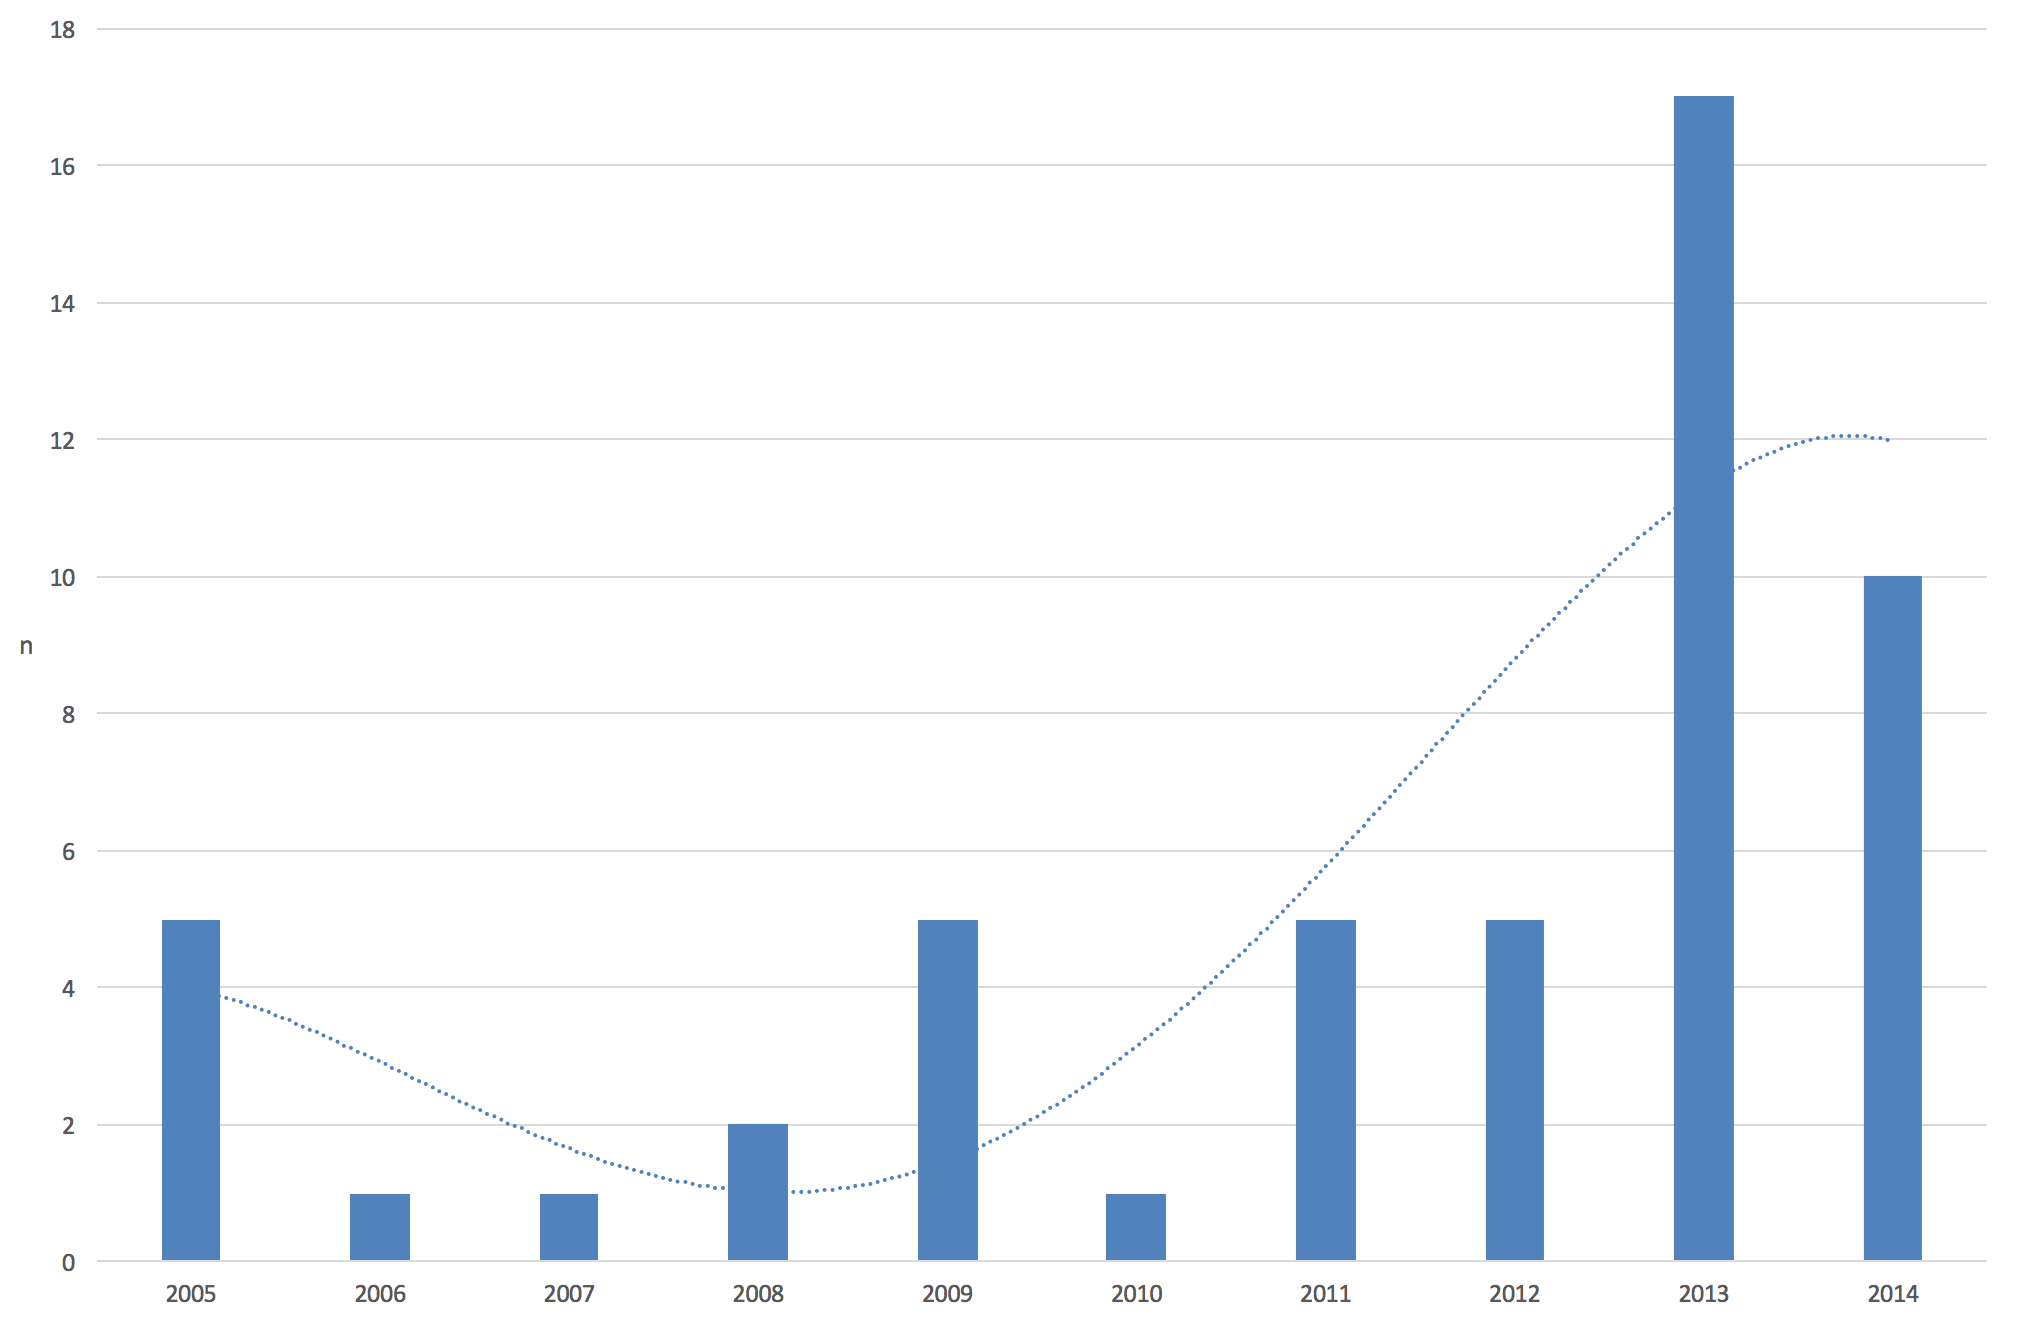
\includegraphics[width=9cm]{img/years}
\caption{Research publications per year.}
\label{fig:years}
\end{figure}


RQ9

Selected articles are almost equally divided between international conference proceeding publications and journal or book chapters.
Publication as proceedings of international conferences remains the overall prevalent group.

\begin{figure}[tbh]
\centering
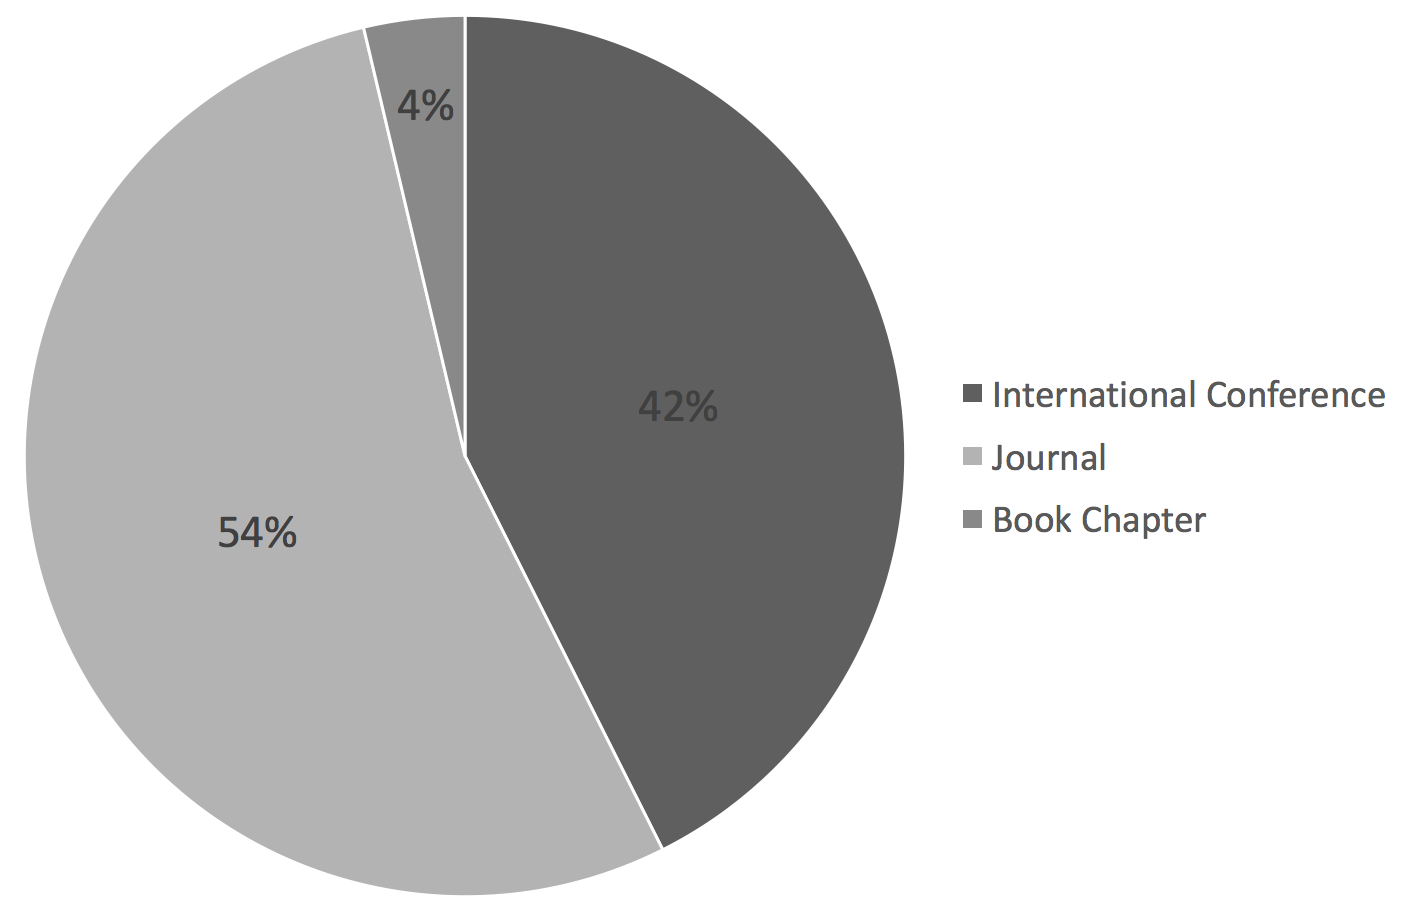
\includegraphics[width=9cm]{img/publication}
\caption{Types of publication.}
\label{fig:publications}
\end{figure}


RQ2 and RQ8

The technological pattern involved in smart-city learning is, most of the times, connected to support the learning process.
For this purpose, the use of mobile devices is the prevailing choice.

Online cooperative platforms of various types are also used in many cases: more precisely e-learning and e-government solutions were mentioned in more than one article.

RQ3
Some articles mentioned specific learning theories applied during the study. Situated Learning\cite{anderson_situated_1996} is the approach that was reported more often.
The approaches that are most often pursued are connected to various levels of collaboration and cooperation between stakeholders or withing the learning community (for example among the students). Context awareness and situatedness are also mentioned in a few articles.

RQ4
Research on smart-city learning often involves case studies oriented to perform some sort of investigation on a specific problem. Solution design or implementation studies are less common, even more rare are studies that make use of IOT, ubiquitous technologies and custom hardware prototyping.

\section{Discussion}
A significant portion of the articles dates back to 2005, this is probably connected to the momentum of the freshly introduced term of \textit{smart} city back in those years, like mentioned in section \ref{sec:intro}.
From the articles screened, some common concepts and research set-ups emerged.
For example several case studies involves schools, students and mobile devices.

A more technological-based approach, for example using custom-built hardware and prototypes, is almost never used.
From the methodological point of view, there seem to be a lack of Design Science\cite{hevner_three_2007} based approach, which would allow to focus more on the technology that fits best the desired learning objectives.

\section{Conclusions}
%insert block diagram schema from PRISMA


%%%%%%%%%%%%%%%%%%%%%%%%%%%%%%%%%%%%%%%%%%%%%%%%%%%%%%%%%%%%%%%%%%%%%%%%%%%%%%%
\bibliographystyle{splncs03}
% \bibliographystyle{IEEEtran}
\bibliography{references_scl}

%%%%%%%%%%%%%%%%%%%%%%%%%%%%%%%%%%%%%%%%%%%%%%%%%%%%%%%%%%%%%%%%%%%%%%%%%%%%%%%

\end{document}
